\documentclass[crop,tikz,border=1px]{standalone}

\usetikzlibrary{arrows,positioning,scopes,automata,calc}

\begin{document}
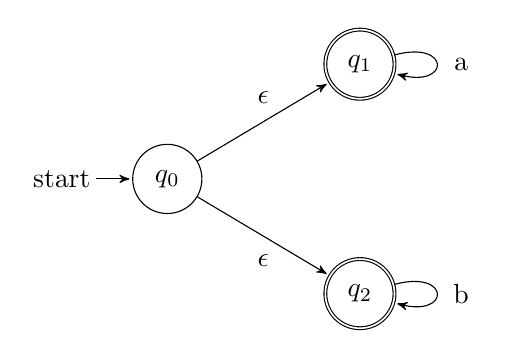
\begin{tikzpicture}[->,>=stealth',shorten >=1pt,auto,node
  distance=2cm,inner sep=2pt,minimum size=.6cm,
  mystate/.style={state,text centered}]

  \node[accepting,mystate] (q1)  {\(q_1\)};
  \node[accepting,mystate] (q2) [below=of q1] {\(q_2\)};
  \coordinate (mid) at ($(q1)!0.5!(q2)$);
  \node[initial,mystate] (q0) [left=of mid] {\(q_0\)};

  \path (q0) edge node [above] {\(\epsilon\)} (q1)
        (q0) edge node [below] {\(\epsilon\)} (q2)

        (q1) edge [loop right] node [right] {a} (q1)
        (q2) edge [loop right] node [right] {b} (q2);

\end{tikzpicture}
\end{document}
